\documentclass[]{../resources/final_report}
\usepackage{graphicx}
\usepackage[hidelinks]{hyperref}
\usepackage{amsmath}
\DeclareMathOperator*{\argmax}{argmax}


%%%%%%%%%%%%%%%%%%%%%%
%%% Input project details
\def\studentname{Roger Milroy}
\def\reportyear{2019}
\def\projecttitle{Autonomous Micro Air Vehicles: Enhanced Navigation in GPS denied environments.}
\def\supervisorname{Professor Sara Bernadini}
\def\degree{BSc (Hons) in Computer Science (Artificial Intelligence)}
\def\fullOrHalfUnit{Full Unit} % indicate if you are doing the project as a Full Unit or Half Unit
\def\finalOrInterim{Interim Report} % indicate if this document is your Final Report or Interim Report

\begin{document}

\maketitle

%%%%%%%%%%%%%%%%%%%%%%
%%% Declaration

\chapter*{Declaration}

This report has been prepared on the basis of my own work. Where other published and unpublished source materials have been used, these have been acknowledged.

\vskip3em

Word Count: 

\vskip3em

Student Name: \studentname

\vskip3em

Date of Submission: 

\vskip3em

Signature:

\newpage

%%%%%%%%%%%%%%%%%%%%%%
%%% Table of Contents
\tableofcontents\pdfbookmark[0]{Table of Contents}{toc}\newpage

%%%%%%%%%%%%%%%%%%%%%%
%%% Your Abstract here

\begin{abstract}

%% Intro to the project



\end{abstract}
\newpage

% %%%%%%%%%%%%%%%%%%%%%%
% %%% Project Spec

% \chapter*{Project Specification}
% \addcontentsline{toc}{chapter}{Project Specification}
% Your project specification goes here.

%%%%%%%%%%%%%%%%%%%%%%
%%% Introduction
\chapter{Introduction}


%%%%%%%%%%%%%%%%%%%%%%
%%% 
\section{Motivation}

Micro Air Vehicles (MAVs), popularly known as quadcopters, have become ubiquitous in recent years with prices dropping across a range of sizes of drones 
which has lead to their deployment across a number of sectors and applications. These include 
videography, where most of us will have seen their output, all the way to 
assessing and counting endangered species.

There are several key challenges operating with MAVs,
primary among these is payload and power constraints, both of which limit onboard computation. 

A second challenge is that of fixing position accurately. Most solutions use some kind of 
satellite navigation solution to fix absolute position. This is effective in outdoor environments
but ineffective in a number of environments. In these environments it is necessary to rely on
inertial sensors as well as image data. These are fused in a Kalman Filter to produce a single
estimate of position.

In order to overcome these joint issues, one solution is offboard computation. This is the 
approach used by Engel, Sturm and Cremers. They communicate with an offboard laptop
which does the heavy computation. This however obviously introduces other issues
such as range and latency. 


%%%%%%%%%%%%%%%%%%%
%%% Objectives
\section{Objectives}

The main objective is to apply the newly proposed technique of Hybrid Inference \cite{Satorras2019CombiningGA} on the
problem of position estimation in MAVs. Hybrid Inference integrates existing models existing models with Neural Networks
in order to improve inference performance in both low and high data regimes.

In addition I aim to demonstrate it using onboard computation, taking position estimates that come from inertial sensors and visual SLAM systems. Using a Jetson Nano for computation, mounted to a DJI Matrice 100 quadcopter.

If I am successful this project could improve the performance of existing navigation solutions 



The overall objective of the project is to implement a new technique first introduced in Combining Generative and Discriminative Models for Hybrid Inference \cite{Satorras2019CombiningGA} in the context of Drone Navigation without GPS.
The second objective is to demonstrate the technique using only onboard computation, for which I will use the Jetson Nano, mounted on the Matrice 100 drone platform. This is to demonstrate an untethered autonomous drone that can navigate accurately without GPS.

For the first term, the key objectives are to validate the technique by implementing it on a small synthetic dataset, to demonstrate in Gazebo the Monocular SLAM with scale recovery technique \cite{Engel:Camera-basedNav} upon which the Hybrid Inference will be implemented and finally to validate the Jetson Nano platform for computation.
The strategy is to ensure that all the major components are in place for the final implementation. There are three strands to the project as a whole, hardware, the TUM developed technique and Hybrid Inference.
For full success of the project, all need to be successful but to demonstrate the core technique only the TUM and Hybrid Inference sections need to function. This drove the objectives for the first term and I decided to leave the hardware integration until next term to maximise the chances of full project success.

The objectives for the second term are to implement Hybrid Inference for state estimation completely and demonstrate it on a simulated quadcopter in Gazebo. Secondary goals are to integrate the Jetson Nano onto the Matrice 100 and adapt the code to work with the DJI OSDK. Finally to demostrate the technique.

%%%%%%%%%%%%%%%%%%%%%%
%%% Planning and Timescale
\chapter{First Term Planning}

\section{Original Plan}

The original plan delayed much of the serious implementation until the second term. While this was not unreasonable given the learning curve for each of the technologies involved, if I stuck to the original plan I would have been faced with a huge amount of work with little to base it on.
There was also quite a lot of uncertainty about the state of the TUM codebase. The original assumption was that the code had been written specifically to work with the Parrot AR drone as it was the one they demonstrated \cite{Engel:Camera-basedNav}.
This would have meant rewriting the code to work in ROS and be platform independent. When I found that was not the case it changed the dynamics of the project quite significantly and led to the new plan which I describe in more detail below.

I have included below the original plan Gantt Charts that detail milestones and the associated timescale.
\\
 % Gantt chart?
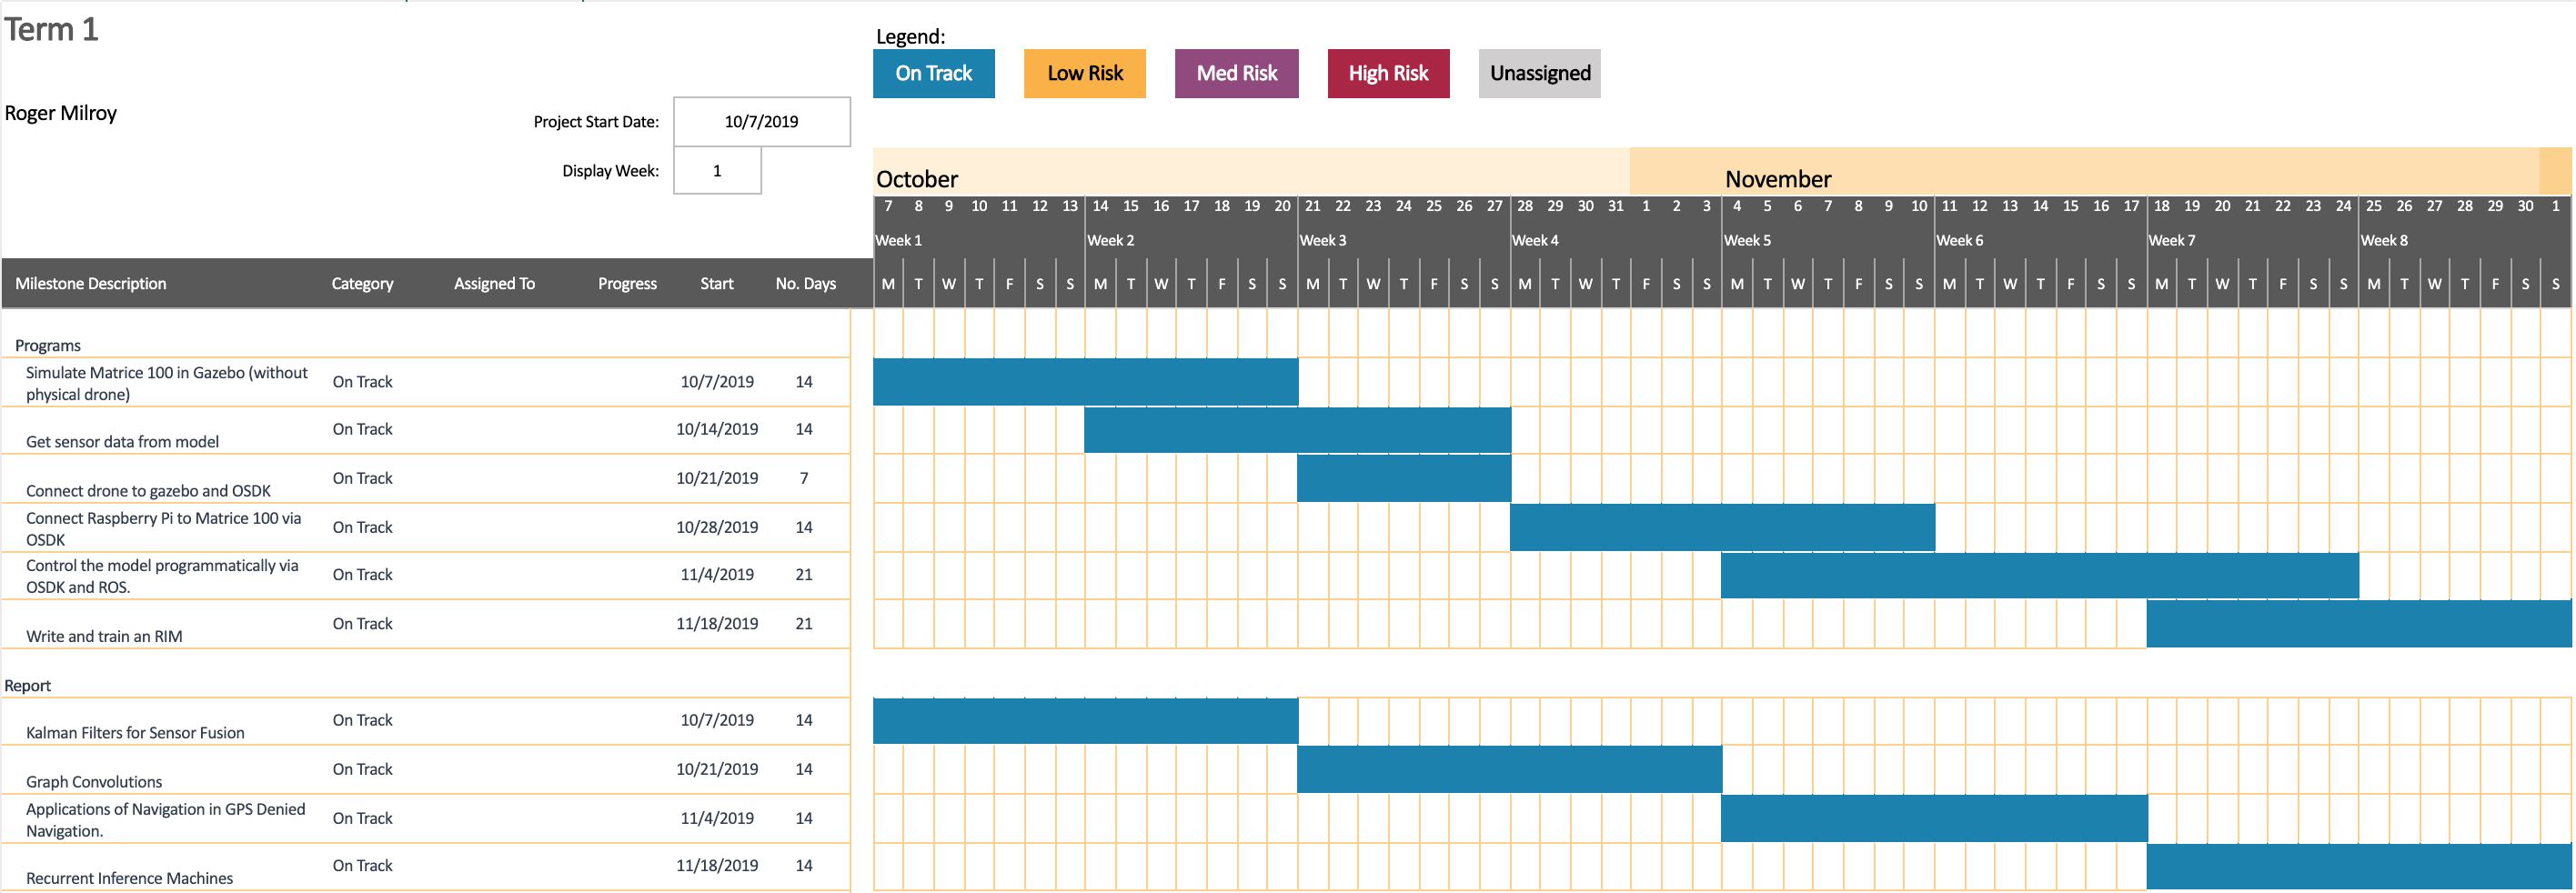
\includegraphics[width=\textwidth]{../resources/images/Term1Ganttv1.png}
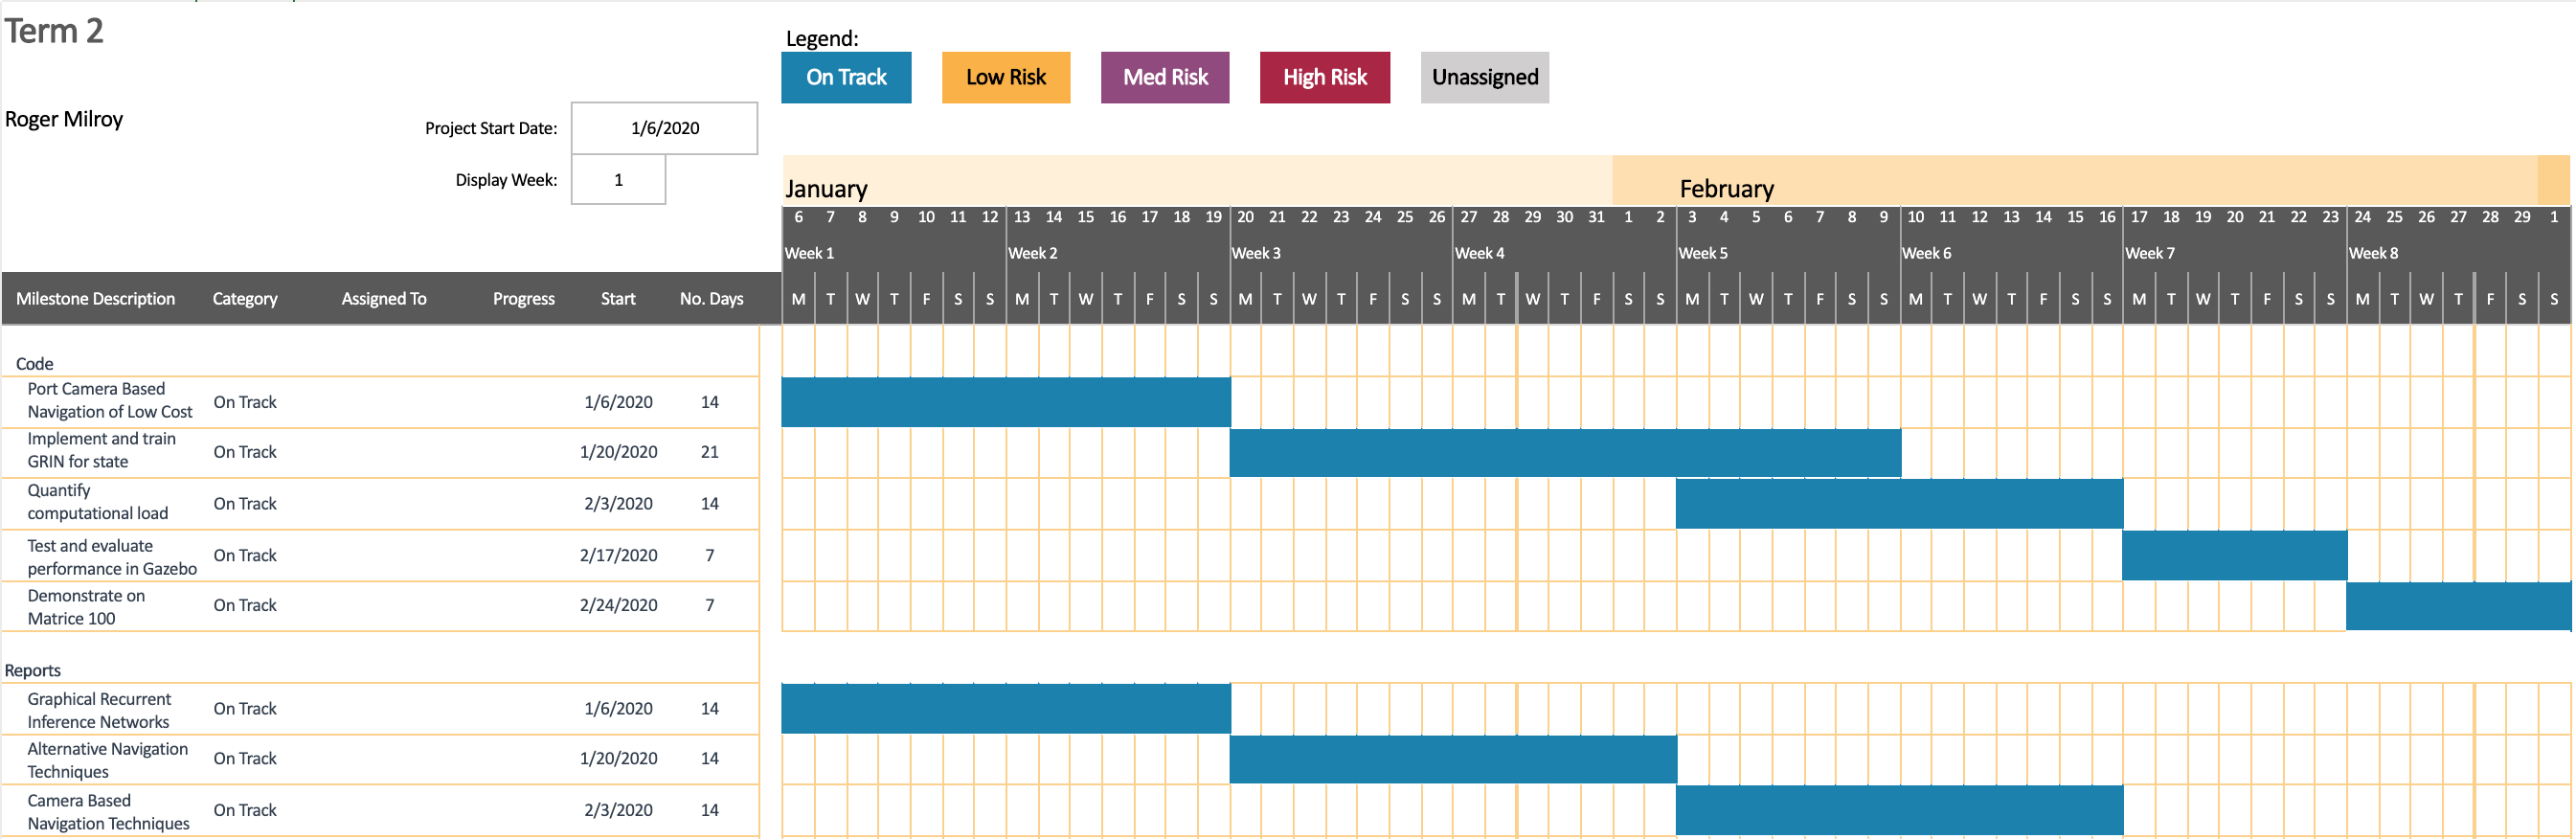
\includegraphics[width=\textwidth]{../resources/images/Term2Ganttv1.png}

\pagebreak
\section{Revised Plan}

While working on the project the outlook changed quite significantly when I found the code for the Monocular SLAM with scale recovery was open source. 
This meant that I could directly build upon their work and extend it instead of spending the bulk of the project reimplementing their technique.
This enabled me to pivot to focusing more on the implementation of Hybrid Inference. I now spend most of the first term getting simulation working with the existing code base.
I also implement a simple version of the Hybrid Inference technique on synthetic position data.

The plan for the second term is to implement Hybrid Inference on the true problem, with the true dynamics of the drone. The second term is also mainly for hardware integration.
I am aware that hardware integration is never straightforward so I have planned 

I replanned and the following are the updated milestones and associated dates.

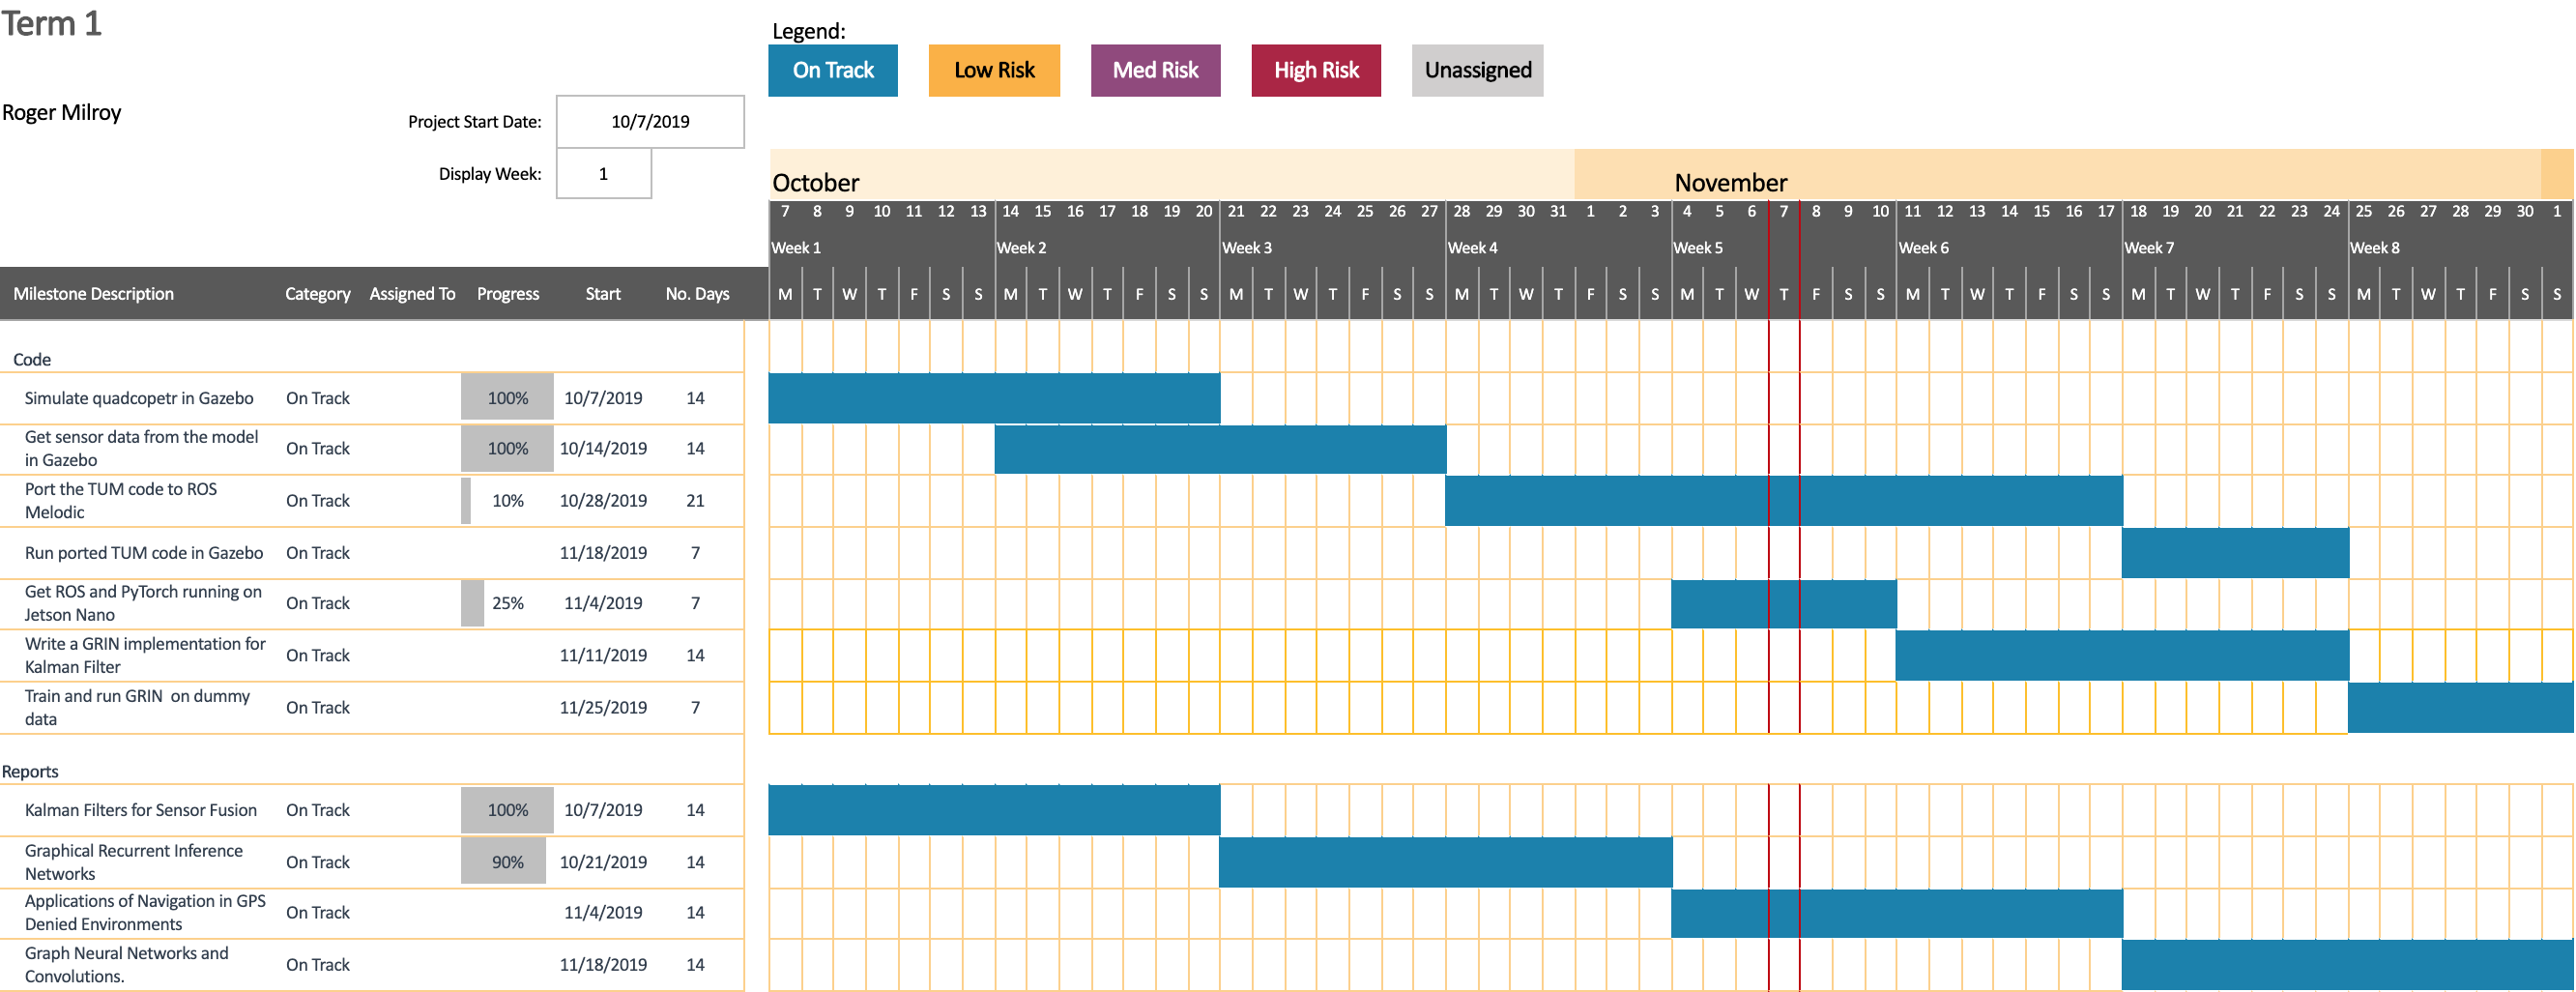
\includegraphics[width=\textwidth]{../resources/images/Term1GanttChart.png}
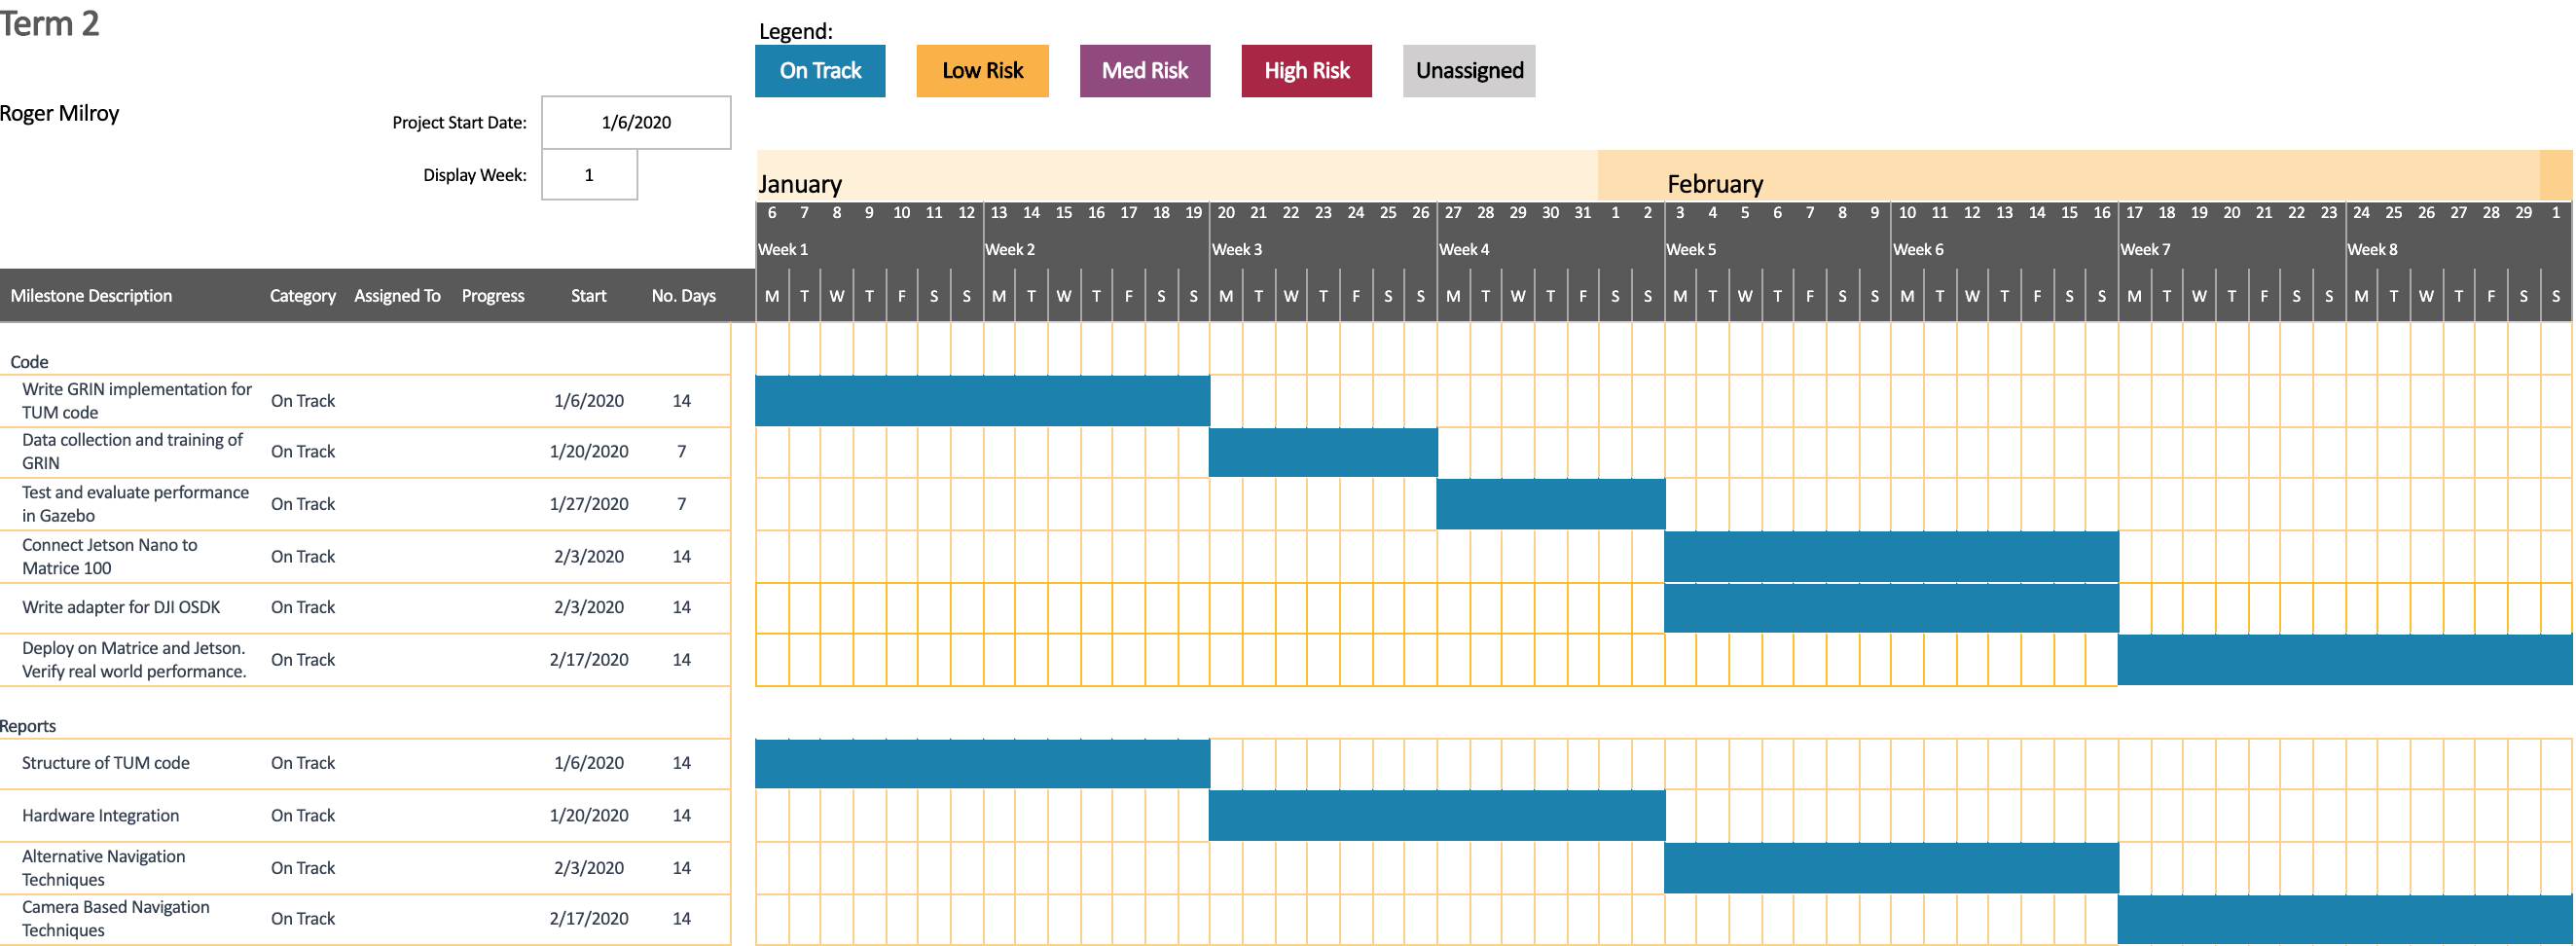
\includegraphics[width=\textwidth]{../resources/images/Term2GanttChart.png}

%%% Software Engineering
\chapter{Software Engineering}

My Software Engineering approach has had to be flexible in this project. I can't apply the same approach to all parts of the project as they each have different requirements and contexts.
Also at this stage of the project there are some aspects that are not relevant to certain sections.

\section{Tools}

\subsection{Version Control System}
I used git as my revision control system, and GitHub as my remote. I actually have a number of repositories because for the ROS section of the project it was necessary to modify existing projects code.
I created a private fork of the relevant projects and then modified them as necessary.

I have separate branches for development, reports and for each feature that I am working on. These last ones are only temporary and are closed as soon as the feature is tested and integrated back into development.
Currently master is reserved for completed sections.

\subsection{Project Task Tracking}
I used Trello in order to organise and keep track of tasks while completing them. I use a single board with To Do, Doing and Done lists. Each task is a card and has an associated due date.
This is really useful to stay on track and quickly assess the state of the project at a glance. I also used this while replanning as I could evaluate each task and see whether it was still relevant in the new context.
One additional advantage of using Trello is that it keeps track of history and has space for lists within tasks allowing them to be broken up into sub tasks.


\subsection{Development Tools}

I used both VSCode and PyCharm as Development Environments. They both have different advantages and disadvantages and I used VSCode for the C++ work and PyCharm for the Python work.

I used the built in testing framework for Python, unittest for testing. This provides a very similar framework to JUnit and allows for clear easy test setup and management.

\section{Development}

\subsection{Design}
% ROS
ROS lends itself to modular code however the packages that I am working with and building on have very mixed engineering approaches.
To date my work has been composing the projects and getting them to run so Software Engineering practices have been limited to thinking about the design of the full implementation.

Unfortunately ROS is not particularly conducive to Test Driven Development (TDD) as there is no framework that enables testing outside of nodes. I can test the components of each node in the standard fashion, which I plan to do though this will apply more next term.

All of the design decisions that I have taken, both for implementations this term and the plans for future work, have been in the pursuit of modularity.

Good code should be modular and reuseable where possible. There are aspects where this is obviously not possible, such as configurations and any implementation specific work, but this should where possible be isolated and offer abstrat interfaces.

With respect to the packages I have chosen, the hector stack and the TUM work, they have to some extent taken this approach but only really within the project. 
This complicates my work somewhat but at the same time using these as the base allows me to explore more advanced concepts over reimplementing the functionality of these modules.
I will be writing adapters to enable the existing codebase to interact.

For the proof of concept of Hybrid Inference, the Dataset and the Linear Motion Model that creates synthetic data I implemented them as separate classes. A standard Object Oriented approach and used composition where necessary.


\subsection{Testing Strategy}

Due to the limitations that I have regarding support for formal testing, I have relied a lot on sanity checking at each stage while testing formally as many sections as possible.
Integration tests are particularly important for my project as I have a variety of different technologies that need to work together across a number of interfaces.
This will become much more important in the next stage of the project as that is when the different components start to interact and when I will be looking to start deploying code onto the hardware.

To this point I have Unit Tested thoroughly the proof of concept of the Hybrid Inference, the Dataset and Linear Motion model.

\subsection{UML}
%% UML
The UML for the Hybrid Inference section of my project is below.

The UML that constitutes the high level architecture of the final project is below.



%%%%%%%%%%%%%%%%%%%%%%
%%% Literature Review
\chapter{Background Theory}
% This is where the background theory will go too.

\section{Gazebo and ROS}

%% Explainer on Gazebo and ROS and see if there are references for them.
In order to demostrate the effectiveness of the code that I have written it is essential that it is demonstrated first in a simulated environment.
This neccesitates using Gazebo as the industry standard robot simulation software. In a similar token the industry standard robot development framework is ROS, which works with Gazebo and so this is the primary technology stack that I am using.

Both ROS and Gazebo are very powerful but they don't have a particularly easy onboarding process. For learning basic ROS concepts I used a service called Robot Ignite Academy that has some simple tutorials to make the process of learning the ROS way of doing things a bit quicker.
One challenge I had at the very early stage was understanding what ROS actually was. There are very few high level descriptions of it, and they are certainly not the first topic on the ROS tutorials pages.

In a nutshell, what I learned was that ROS is a paradigm of programming robots as well as an implementation of that paradigm. The paradigm is that each peice of code on the robot is a Node that takes data from a Topic, processes it and outputs data for other Nodes to use on a Topic. 
Some Nodes don't do both of these and some also directly effect change in the robot, think of a Node that controls a motor, it would read and change the voltage to the motor.

The other concepts that make up ROS are that of Services which are synchronous and Activities that are asynchronous, both operate on the Client - Server pattern. Topics as I mentioned are communication channels that operate on the Publisher-Subscriber pattern. And Messages which actually have quite a bit of intricacy and can be quite confusing.
There are 3 types of Message. Regular Messages that are published to Topics. Then Actions and Services also define their own formats of messages. They will often use standard messages defined for use in Topics but additional message formats will be generated for each Action or Service.
%% Need to add references


\pagebreak
\section{Monocular SLAM with scale recovery.}

%% put a UML diagram of the library layout/dependancies.
In two related papers, Engel et al. present a technique of monocular Simultaneous Localization and Mapping (SLAM) that is able to recover absolute scale. In order to understand why this is significant and important some background is needed.

The primary problem of visual SLAM techniques is that of creating a high quality depth map of the surroundings. This can be accomplished by stereo vision, which is where two cameras are used and the distance and rotation between the two of them are known. Ideally the axes are aligned and there is no rotation between the cameras though this can vary depending on the specific requirements.
This can be extended to use three or more cameras but in the more general case, known as structure from motion, it is possible to use a single camera and in that case we are trying to recover the transformation and rotation between frames. This is possible however it is not possible to recover absolute scale from this technique as we don't know the absolute distances between frames. In the stereo case the information about the position and orientation of the cameras relative to each other is known a priori and so we can recover absolute scale.

Engel et al. tackle the issue of scale recovery by using data from the Inertial Measurement Unit (IMU) which usually consists of 3 accelerometers and 3 gyroscopes and often a magnetometer or other absolute scale sensors such as altimeter or barometer.. This is very standard on quadcopters as it is needed to keep it stable. They use the information provided by this sensor in conjunction with the structure from motion equations in order to recover the absolute scale. 
In order to estimate the scale factor which is usually referred to as $\lambda$ they take a maximum likelihood approach, which in simple terms means they estimate the $\lambda$ that maximises the likelihood of the $x$ and $y$ positions measured by onboard sensors. In order to solve successfully they turn it into the negative log likelihood which you then minimize. This is a common trick and in this case it leads to a closed form solution for $\lambda$. 
This is important as it reduces the computational cost and makes it more feasible with onboard computation. In the paper they use a Parrot AR drone which has very constrained payload and computation capacity so they use offboard computation.

In the second paper \cite{Engel:FigureFlying} they present the full system including the scale estimation and demonstrate its effectiveness in position flying and holding.


\pagebreak
\section{State Estimation}

%% Kalman Filters
The core method used for state estimation in the face of noisy sensors is the Kalman Filter. It is used by Engel et al.\cite{Engel:Camera-basedNav} for state estimation and sensor fusion which are its most common uses in this field.

Let us formally define the problem. The system we are measuring is assumed to be characterised by a Hidden Markov Model, this is how Kalman characterised the dynamical system we are interested in \cite{Kalman1960ANA}. 
In this formulation there are hidden states $x$ and observations $y$. The system being Markovian means that it is characterised by the following equations:

\begin{align}
  x_t &= Ax_{t-1} + Q_t \\
  y_t &= Hx_t + R_t
\end{align}

Where $A$ is the transition matrix from time $t-1$ to $t$, and $\xi_t$ is the noise at time $t$. This represents that the model dynamics are stationary so $A$ is fixed but there is noise in transitions, that is transitioning between states is non-deterministic.
$H$ is the measurement matrix and $\eta_t$ is the noise in the measurements. This models the reality of noisy measurements that may not be correct and in fact represents the true problem. We want to recover the true measurements despite being given noisy observations.

The Kalman Filter gives an optimum estimate of $x$ which I will call $x^*$ by deriving three matrices $\Phi^*$, $P^*$ and $\Delta^*$:

\begin{align}
  \Delta^*(t) &= A_{t+1;t}P^*_tH^T_t[H_tP^*_tH^T_t]^{-1} \\
  \Phi^*_{t+1;t} &= A_{t+1;t} - \Delta^*_{t+1;t}H{t} \\
  P*_{t+1} &= \Phi^*_{t+1;t}P^*_tA^T_{t+1;t} + Q{t}
\end{align}

Note that in the Kalman formulation he also considers non stationary dynamic systems. In our situation we assume stationarity which allows us to drop the time specification on the transition matrices $A$ and $H$.

With these matrices, the optimal estimate of state at time $t+1$, $\hat{x}_{t+1|t}$ is given by 

\begin{align}
  \hat{x}_{t+1|t} &= A^*\hat{x}_{t|t-1} + \Delta^*_ty_t
\end{align}

The estimation error $x'$ and covariance of the error, cov $x'$ are

\begin{align}
  x'_{t+1|t} &= A^*x'_{t|t-1} + Q_t \\
  \text{cov } x' &= P^*_t
\end{align}

From this we can see that the Kalman Filter is an iterative process where each iteration builds upon the previous best estimate of state.
To recover the estimates of the true measurements we simply need to multiply the best estimates of the state by the measurement matris $H$.

Kalman and Bucy extended the Kalman filter that above stated works for discrete time, to the continuous case the year after the original paper \cite{Klmn1961NewRI}.

These equations only apply to linear dynamic models which is something of an issue given that most real life applications are of non linear dynamic systems. Thankfully we can use Taylor expansions to linearise our non-linear models around the current state \cite{ExtendedKalmanNasa}. 
This does unfortunately add a large overhead as we need to re linearise at each time step to avoid accumulating linearisation errors.

%% Hybrid Inference
\section{Hybrid Inference}

Now I introduce the technique that form the core objective of this project, Hybrid Inference. First introduced in \cite{Satorras2019CombiningGA} which also gave examples on Lorenz attractors and Kalman filters.
While Kalman Filters give optimal estimates in the face of noise, it is almost impossible for them to be completely precise due to that noise. This we can see by observing the error in the estimates at each time step.

Absent an accurate fix of state, ie. a noiseless measurement, the error and it's covariance grow continuously to the point where estimates may no longer be meaningful.

At the same time it is now possible to train a neural network to directly estimate position given noisy inputs, as shown by Yadaiah and Sowmya\cite{NNStateEstimation}. The concept of Hybrid Inference is to leverage the relative strengths of pre-existing knowledge, in this case the Kalman Filter that accurately describes the behaviour of linear or linearised dynamic models up to a degree of error, and Deep Learning techniques that are able to model highly non linear systems but require large amounts of data to train.
In the Hybrid Inference model, expert knowledge is incorporated by integrating the model of the system with a GNN modelling the residual error to improve accuracy above what is possible with a Kalman filter alone.


Reexamining the problem solved by the Kalman filter, Satorras, Akata and Welling reformulate the problem to be a maximum likelihood problem\cite{Satorras2019CombiningGA}.
Where the states are $\mathbf{x} = \{x_0, x_1 ... x_k\}$ and the observations are $\mathbf{y} = \{y_0, y_1 ... y_k\}$
In this context, the task is to predict the optimal estimate of $\mathbf{x}$, $\mathbf{\hat{x}}$ which is defined as

\begin{align}
  \mathbf{\hat{x}} = \underset{x}{\text{argmax}}\ p(\mathbf{x}|\mathbf{y})
\end{align}

Again as we assume a Markov process and that the transition is stationary this can be expressed as 

\begin{align}
  p(\mathbf{x},\mathbf{y}) = p(x_0)\prod_{t=1}^T p(x_t|x_t-1) p(y_t|x_t)
\end{align}

They model this as an iterative optimization process to arrive at $\mathbf{\hat{x}}$
Specifically they define a recursive update operation for the general case and then formulate it for the hidden Markov case

\begin{align}
  x_t^{(i+1)} = x_t^{(i)} + \gamma M_t
\end{align}

Where $M_t$ represents the sum of matrix products, which they call messages, from $x_t-1$ to $x_t$ from $x_t+1$ to $x_t$ and from $y_t$ to $x_t$.

In our case these messages turn out to be

\begin{align}
  x_{t-1} \rightarrow x_{t} &= -Q^{-1}(x_t - Fx_{t-1}) \\
  x_{t+1} \rightarrow x_{t} &= F^TQ^{-1}(x_{t+1} - Fx_t) \\
  y_t \rightarrow x_t &= H^TR^{-1}(y_t - Hx_t) 
\end{align}

The graphical interpretation is of the $x$s and $y$s at each time step forming nodes in a graph. The edges are the same as the direction of the messages, that is from $x_{t-1} \rightarrow x_t$, $x_{t+1} \rightarrow x_t$ and $y_t \rightarrow x_t$.The messages passed over these edges iteratively update the $x$s and after some iterations they converge to a best estimate.

%% Insert a graph here.

This graphical interpretation allows us to define an equivalent graph with different dimension nodes but the same edges. These are known as $h_x$ and $h_y$ which stands for hidden nodes relating to $x$ and $y$ respectively. 

%% Insert another graph here.

The key part of the paper is to define a Graphical Neural Network that operates over this graph with a message passing routine over the nodes that connect edges and the messages passed in the original graph. More specifically for each type of edge, for example $y_t \rightarrow x_t$, we define a feedforward neural network that takes the source node, the target node and the message and outputs an encoding of the edge, I will refer to these as edge models.
These encodings are summed according to their source node and then passed through a separate feedforward network which I will call the node model. The output of this is passed through a GRU (Gated Recurrent Unit) along with the previous $h_x$ in order to produce a new estimate of $h_x$.
The interpretation of this is that edge feedforward networks compute the residual error over the edges, the node model computes the residual error left in the $h_x$ and the GRU allows some of the past residual error to propagate into the current estimate.

The final step passes the new $h_x$ through a decoding step to produce an additional corrective factor in addition to $M_t$ called $\epsilon$.

This gives us the final general recursive update rule

\begin{align}
  x_t^{(i+1)} = x_t^{(i)} + \gamma (M_t + \epsilon_t)
\end{align}


%% Graph Neural Networks in this context


%%%%%%%%%%%%%%%%%%%%%%
%%% Work Completed
\chapter{Work Completed}

%%% Written Summary
\section{Summary}
\subsection{ROS and Gazebo}

%% install ROS and Gazebo
The first task to carry out was to install ROS and Gazebo. As mentioned earlier ROS is the framework into which my code will fit. Gazebo is a simulation tool that I will be using to verify everything before deploying anything in reality.
Luckily Gazebo is included with ROS (with some exceptions) so installing it separately is not necessary. If you need the most recent version of Gazebo this is not true, you need to follow some additional steps to install it and link it with ROS so they interact correctly.

I did have some confusion about which version of ROS I needed to be compatible with various things but I made the decision to stick with the most recent version of ROS and the standard version of Gazebo packaged with that. This simplifies the setup for anyone seeking to reproduce my project.

The ROS website\cite{melodic/installation/ubuntu} has an excellent guide on installing ROS for the first time on Ubuntu and I highly recommend it.

%% install hector code

%% explain catkin workspace.

After that I installed the hector stack. This was quite a long process of trial and error as there does not seem to be a guide for getting started with this set of packages.
I first tried to install them from apt as they are available there. That did not work and I believe the issue is that they were built for an earlier version of ROS but packaged for melodic without any changes. Regardless of the reason that did not work. 
I was trying to install the hector quadrotor and hector gazebo packages as those were the only packages that I believed that I needed. I tried to clone them into the src folder of my catkin workspace.
While trying to build it failed because of dependencies on other hector packages, namely hector slam hector models and hector localization. Then it was missing the geographic mesages. Then it failed because it was missing qt4. I installed both of those with apt. The full process took a while longer than this explanation as you only find out anpther dependency is missing after building again.
A final issue was that the memory usage at certain points spikes. It turned out that this was causing the VM to run out of memory and stop compliation. This caused very confusing error messages as they didnt seem to be for anything in particular. I finally figured out with the help of htop and allocated more memory to the VM which solved the issue. One anachonism of this stack is that it doesn't seem to build in the right order. 
It will often fail only to complete more after rerunning. At one point it was necessary to continually rerun catkin\_make about 7 or 8 times in a row. You only get concerned when it stops at the same percentage built more than once. 


%% 

\subsection{Hardware}

%% evaluation of alternatives
My original plan was to use the Raspberry Pi for the onboard computation when I transition to operating on the physical drone rather than in Gazebo.
This was for a couple of reasons, primary was the low power draw while still offering gigahertz computation. I have a Raspberry Pi 2 and I planned to purchase a Raspberry Pi 4 for the final implementation due to its increased compute power.

%% selection of Jetson Nano
While experimenting with my RasPi 2 I found some limitations with its implementation of Python as well as concerns about its prospective performance due to reports found online.
I researched alternatives, as there are a wide variety of Single Board Computers on the market now. While looking I found that Nvidia produce the Jetson Nano and specifically the SDK kit, which is very similar to the RasPi but has native support for PyTorch, the deep learning library I am using as well as having 128 GPU cores.
This enables me to take advantage of parallelised matrix computation with the associated performance improvements. On top of this it only consumes up to 10W of power, admittedly this is double the 5W draw of the RasPi but 10 is the maximum, not necessarily what it will consume. I will explore power consumption in the second part of the project.

%% installation of PyTorch and ROS.
After the Nano arrived I installed PyTorch and ROS onto it. This allowed me to verify the steps needed for installing both packages and ensure the most streamlined set of instructions.


\subsection{TUM code}

%% Go through the process. Look at the diary.
The first step in working with the TUM code was to compile it. I was aware that it was written to target ROS xxx which is X versions behind Melodic.

I first attempted to build the project on the Jetson Nano as I was planning to use it as my development platform as well as the deployment environment if possible.
This was not possible. The build failed due to a dependancy, ardrone\_autonomy. This is a wrapper for the Parrot AR drones SDK. It also provides a number of message definitions.
I attemped first to build the dependancy on the Nano but there are issues with compiling that code on an ARM platform. This prompted me to drop the dependancy and the speed of compilation prompted me to abandon the Nano for development.

I found that the only code from the ardrone\_autonomy package were the messages. I then extracted the message definitions from the ardrone\_autonomy package into my own package.

After solving that issue I ran into much more serious issues with a third party library called libcvd which is an OpenCV alternative that PTAM, the monocular SLAM component. (refer to the package diagram.)
This package is packaged as a thirdparty library inside a tarball with two other libraries.
Upon building it would fail on apparently legal C++ code. I tried to use the most recent version of libcvd, pulling it from github, building and installing it on the system separately. This didn't work so I tried placing it into the thirdparty tarball.
That also didn't work. I found that the directory structure of the new version did not match the original and there was a Makefile I needed to replicate. I then found that there were some files that had been deprecated but the TUM code relied upon so I pulled them over from an old version of the library.
This on it's own did not fix the issue but when I found a final Makefile I could add the files I had pulled over into the list of artifacts that would be made available by that stage of the build. 

Then I found some namespace issues as another dependency was not being found in the expected manner. I had to set a definition in order to fix that problem.
I also had to remove the GUI section of the code as it had more serious persistent issues. If I have time spare after completing the project I will go back and try and fix that as well.
Finally there was a section of code that relied upon tf, which is a geometry package of ROS but is now deprecated. I had to rewrite that section to use tf2 which is the replacement.

After building it ran without issue.

I then had to get it to interact with the hector stack. I looked through the hector stack and it is very large. A lot of it is not needed for my project so I considered extracting the core functionality that I want, create a world with a quadcopter that acts correctly.
Unfortunately the hector stack has a large number of interdependencies so it is infeasible to extract only certain components, at least not at this stage.
I have identified where they will interface. They use different conventions for positions so I need to create an adapter.

\subsection{Hybrid Inference}

%% Create the dataset
\subsection{Data}
% understand the linear models, create one (discrete vs non discrete)
A prerequisite for any task that includes neural network is collecting or creating the data for it to train on.
In this case my dataset is created as at this stage I am firstly verifying that the technique works as expected and I can implement it.
After this stage I will formulate the real problem and collect data in Gazebo for that stage.

My dataset consists of position data generated by a simple linear model with Gaussian noise in the transition matrix as well as the measurement matrix.
This is very similar to one of the experiments carried out in the original paper \cite{Satorras2019CombiningGA}. This is intentional in order to have comparison data, though the model I am using is likely to be much simpler than that used in the paper.

% testing
The testing strategy I have used for the Linear Model and the Dataset is designed to verify the core performance.
That the amount of data created is correct, that the various options operate as expected and that the output data is in the format expected.

%% Create the Kalman filter
% understand and formulate
\subsection{Graphical Model, GNN and Hybrid Inference}

My original understanding of the Hybrid Inference formulation was that the graphical model was a regular Kalman Filter and the GNN was formulated in a similar fashion.
As I describe above that is not the case, the graphical model is a reformulation of the problem and solution. 
I realised this after reading the paper with reference to the GitHub repository with their implementation \cite{vgsatorrasgithub}. It took a fairly long time to understand their code as it is not really documented and has a somewhat confusing structure.

Implementing the graphical model was then relatively straightforward though trying to keep it self contained and modular complicated things slightly. 
My implementation of the GNN is quite problem specific. At the moment I can't see much way to make it more generic. Given that I will have to reformulate for the reasons just stated I will explore where the commonalities are and whether a generic version is feasible or desireable.
It differs quite a lot from the Satorras' formulation mainly due to my desire to improve the interpretability of the code and give a cleaner flow and structure. Functionally they are equivalent except that my node model is a 3 layer feedforward network where theirs is 2 layers.
I also decided not to implement different modes for graphical only or GNN only as I specified these as separate standalone, or semi standalone in the case of the GNN, classes.

As I had implemented the two components separately it made the Hybrid Inference very simple as it is just a composition of the two.

The current implementation really implements a Kalman Smoother, that is an optimal estimate of past observations, not a real time filter or predictor which is really what is needed for the full realisation of this project.

The key challenge in extending it to the realm of prediction is the fact that some of the messages will become meaningless, particularly the $y$s or observations that we have not observed yet. It is possible that using zeros is a possible solution though it is not certain.

Another challenge that came up in this section of work is the fact that the Hidden Markov process that I am modelling is slightly different to the one evaluated by Satorras et al.
The state transition they evaluate is 
\begin{align}
  x_t &= Ax_{t-1} + Q_t
\end{align}

But the state transition for a drone will actually be
\begin{align}
  x_t &= Ax_{t-1} + Gu_t + Q_t
\end{align} 

Where $G$ is the input gain matrix and $u_t$ is the input at time $t$.
This is not a problem but it will require me reformulating the graphical model and the respective messages. This is not something that I had anticipated so this will figure into my plans for next term.

%%%%%%%%%%%%%%%%%%%%%%%%%%%
%%% 
\chapter{Second Term Plans}

%%% Hybrid Inference
% work out the formulation and implement for the case of the quadcopter

%%% ROS and Gazebo


%%% Hardware


%%% Diary Section
\section{Diary}

% TODO put some selected extracts from the diary. make an appendix.

%% actually just put all of the diary... Need to format so it isnt shit.

%%%%%%%%%%%%%%%%%
%%%% BIBLIOGRAPHY

\newpage
\bibliographystyle{acm}
\bibliography{../resources/final_project}
\nocite{*}

\label{endpage}

\end{document}

\end{article}